\chapter{Programmierung des Lego Mindstorms NXT}
\label{chap:Lego-Framework}

% Auflistung
% Analyse 
% Auswahl: LeJos

\section{Programmierung}

Die Programmierung des NXT findet mittels der Entwicklungsumgebung NXT-G statt. Hierbei handelt es sich um einen grafischen Editor, mit dessen Hilfe die Logik des Roboters umgesetzt werden kann. Die Sensoren und Aktoren des Lego Roboters werden als Bl\"ocke dargestellt, \"uber die verschiedene Einstellungen vorgenommen werden k\"onnen. Weitere Bl\"ocke unterst\"utzen simple Programmlogiken wie Schleifen und Bedingungen. Hiermit soll das Blockbausystem von LEGO immitiert, sowie ein leichter Einstieg in die Programmierung des Roboters geschaffen werden. In Abbildung \ref{fig:nxtg} ist ein Ausschnitt eines Programms in der graphischen Oberfl\"ache des Editors zu sehen.

\begin{figure}[htb]
\centering
%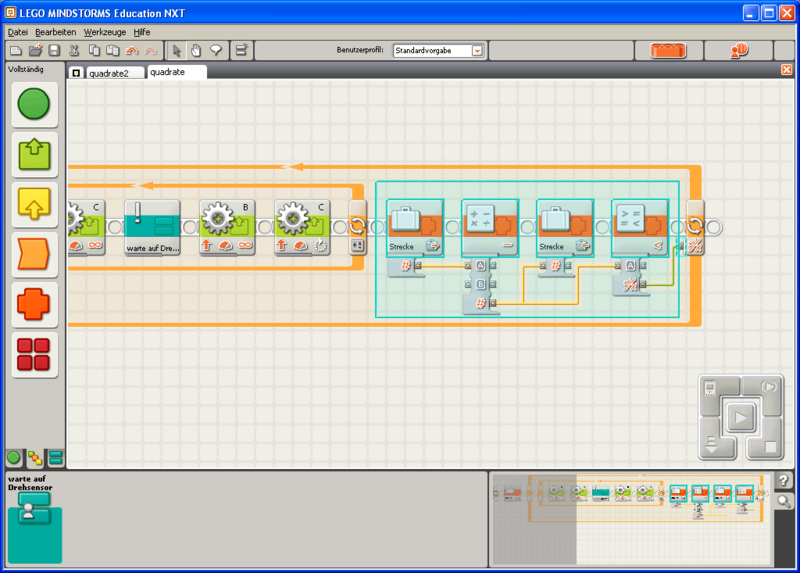
\includegraphics[width=0.8\textwidth]{img/nxtg/800px-Mindst-eblock4.png}
\caption[Skeleton]{Oberfl\"ache der Entwicklungsumgebung NXT-G (Quelle: debacher.de/wiki/NXT-G.\footnote{\href{http://www.debacher.de/wiki/NXT-G}{\textit{NXT-G}} debacher.de, Abgerufen Mai 22, 2013})}
\label{fig:nxtg}
\end{figure}


\par\smallskip 
Mit Hilfe dieser Anwendung ist zwar eine leichte Programmierung des NXT m\"oglich, ist aber f\"ur dieses Projekt nicht sinnvoll einsetzbar. Die Firmware des NXT, sowie die Spezifikation der Sensoren und Aktoren, wurden von Lego ver\"offentlicht. Dar\"uber hinaus auch diverse Developer Toolkits. Durch diese Unterst\"utzung sind eine Vielzahl an Frameworks in verschieden Programmiersprachen und Umgebungen entstanden mit denen der NXT-Baustein programmiert oder auch aus der Ferne gesteuert werden kann.

\section{Auswahl eines Frameworks}

In dieser Arbeit soll nach M\"oglichkeit eine Umsetzung in der Programmiersprache Java erarbeitet werden. In der nachfolgenden Tabelle \ref{tab:NXT_Sprachen} ist eine Auswahl an Frameworks zu finden, welche eine solche Umsetzung in der gew\"unschten Sprache erlauben.
\par\smallskip
\begin{table}[H]
\label{tab:NXT_Sprachen}
\caption[Java Frameworks zur Programmierung des NXT]{ Java Frameworks zur Programmierung des NXT\footnote{\href{http://en.wikipedia.org/wiki/LEGO_Mindstorms\#Programming_languages_2}{\enquote{Lego Mindstorms - Programming languages}}. en.wikipedia.org. Abgerufen Mai 22, 2013}}
\begin{tabular}{|p{5.7cm}|p{9cm}|}
\hline
\textbf{Framework} & \textbf{Sprache} \\
\hline
NXTGCC\footnote{\href{http://nxtgcc.sourceforge.net/}{\enquote{NXTGCC}}. nxtgcc.sourceforge.net. Abgerufen Mai 22, 2013} & C/C++, Objective-C, Fortran, Java, Ada, others \\
\hline
leJOS\footnote{\href{http://lejos.sourceforge.net/}{\enquote{leJOS}}. lejos.sourceforge.net. Abgerufen Mai 22, 2013} & Java \\
\hline
TinyVM\footnote{\href{http://tinyvm.sourceforge.net/}{\enquote{Tiny VM}}. tinyvm.sourceforge.net. Abgerufen Mai 22, 2013} & Java \\
\hline
Gostai Urbi\footnote{\href{http://www.urbiforge.org/index.php/Robots/Mindstorms}{\enquote{Gostai Urbi - Mindstorms}}. urbiforge.org. Abgerufen Mai 22, 2013} & URBI, C++, Java, Matlab \\
\hline
\end{tabular}
\end{table}

\par\smallskip

Durch das erste genannte Framework NXTGCC, also einen Compiler, ist die Programmierung des Bausteins auf einer sehr hardware-nahen Ebene m\"oglich. Dies bedeutet jedoch auch einen sehr hohen Aufwand bei der Umsetzung des vorhabens.
\par\smallskip
leJOS ist ein sehr ausgereiftes Framework zur Programmierung des NXT mit Java. Der Code wird auf einer eigens entwickelten Firmware auf dem NXT ausgef\"uhrt. Außerdem ist auch Codeausf\"uhrung von einem Computer m\"oglich. Da dies das Framework ist, welches zur Verwendung in dieser Arbeit ausgew\"ahlt wurde, wird es im nachfolgenden Kapitel n\"aher beschrieben.
\par\smallskip
TinyVM kann eigentlich von vorneherein ausgeschlossen werden, da es sich nur zur Programmierung des RCX Bausteins von Lego handelt. Es wird hier jedoch trotzdem erw\"ahnt, da der RCX der Vorg\"anger des NXT ist, sowie auch TinyVM der Vorl\"aufer des zuvor genannten NXT darstellt. Wie auch bei leJOS bringt TinyVM eine eigene Firmware f\"ur den Lego Roboter mit.
\par\smallskip
Urbi ist kein eigenes Framework zur Ansteuerung des Lego Roboters selbst, sondern eine Open Source Platform die sich der Steuerung von Robotern und komplexen System im allgemeinen zuwendet. F\"ur den NXT existiert hier eine Schnittstelle. Da es sich hier um ein großes Framework mit sehr weitem Anspruch handelt wird von der Verwendung dieses Frameworks abgesehen.

\section{leJOS - Java for LEGO Mindstorms}

leJOS bietet eine breite Palette an Tools zur Programmierung des NXT mit der Programmiersprache Java. leJOS ging als Open Source Projekt aus TinyVM hervor, welches von Jos\'e Solrzano entwickelt wurde. Kern von leJOS ist die Umsetzung der Java Virtual Machine auf dem NXT Baustein. Diese ist notwendig um Java Code \"uberhaupt erst auszuf\"uhren. Die umgesetzten Features werden auf der Website wie folgt beschrieben\footnote{\href{http://lejos.sourceforge.net/nxj.php}{\enquote{NXJ - Technologie}}. lejos.sourceforge.net. Abgerufen Mai 22, 2013} :

\begin{itemize}
  \item Object oriented language (Java)
  \item Preemptive threads (tasks)
  \item Arrays, including multi-dimensional
  \item Recursion
  \item Synchronization
  \item Exceptions
  \item Java types including float, long, and String
  \item Most of the java.lang, java.util and java.io classes
  \item A Well-documented Robotics API
\end{itemize}

Die erw\"ahnte Robotics API ist die NXJ API. Sie stellt die Schnittstelle zu den Aktoren und Sensoren, sowie den Funktionen des Bausteins, wie beispielsweise Bluetooth, des Lego Roboters dar. Zur Verwendng muss die leJOS Firmware auf dem NXT installiert werden. Dies ist durch mitgelieferte Tools leicht m\"oglich. Zur Entwicklung bringt das Framework ein Eclipse-Plugin mit sich, dies ist hilfreich, da die Entwicklung in diesem Projekt ebenfalls mit Eclipse erfolgt.
\par\smallskip
Die API ist auf zwei Arten realisiert. Einmal zur direkten Verwendung auf dem Baustein und zum anderen zum Ansteuern des NXT aus der Ferne. Es k\"onnen also Programme zur direkten Ausf\"uhrung auf dem Roboter oder \"uber das Remote-Interface, zur Ausf\"uhrung aus der Ferne mittels Bluetooth entwickelt werden. In der Verwendung ist hier keine andere Herangehensweise erforderlich. Es muss lediglich die entsprechend gew\"unschte Implementierung der API verwendet werden. Zur Verwendung der Bluetooth-Kommunikation ist auch kein erheblich großer Aufwand notwendig, dies wird komplett durch das Framework \"ubernommen.
\par\smallskip
Das Framework wurde ausgew\"ahlt, da es viele Funktionen bereits abdeckt und  somit erlaubt, sich im wesentlichen auf das Implementieren der gew\"uenschten Funktionen zu beschr\"anken. Ebenfalls ist die Verwendung in ausf\"uhrlicher Dokumentation geschildert.